%% Bookheader, Nov 8, 2020; July 18, 2022

\documentclass[11pt]{../Support/ourbook}
%% or for landscape, comment out line above and use this one:
%%\documentclass[landscape,11pt]{ourbook}

%% This will keep space from stretching around display math:

\makeatletter
\renewcommand\normalsize{%
   \@setfontsize\normalsize\@xipt{13.6}%
   \abovedisplayskip 11\p@  \@minus6\p@
   \abovedisplayshortskip \z@ 
   \belowdisplayshortskip 6.5\p@ \@minus3\p@
   \belowdisplayskip \abovedisplayskip
   \let\@listi\@listI}
\makeatother
\normalsize


\begin{document}

\tableofcontents
\graphicspath{{../../Chapters/sets/en_US}}
\chapter{Sets and Logic}

The study of math can be basically broken into two purposes:
\begin{itemize}
\item \textit{Developing mathematical tools that let us make better predictions.}  This is how engineers and scientists use math.  It is usually referred to as \newterm{applied math}.
\item \textit{Creating interesting statements and proving them to be true or false.}  This is known as \newterm{pure math}.
\end{itemize}

A lot of mathematical ideas start out as pure math, and eventually
become useful.  For example, the field of number theory is devoted to
proving things about prime numbers.  The mathematicians who created
number theory were certain that it could never be used for any
practical purpose.  After a century or two, number theory was used as
the basis most cryptography systems.

Some ideas start out as a "rule of thumb" that engineers use and are
eventually rigorously defined and proven.

This course tends to emphasize applied math, but you should know
something about the tools of pure math.

All of mathematics is built on a very small and simple foundation:\index{axiom}
\begin{itemize}
\item The idea of a set.
\item A short list of axioms defined in terms of sets. (An \newterm{axiom} is statement that we just accept as true.)
\item A few rules of logic.
\end{itemize}

There have been several efforts to codify a small but complete
axiomatic system. The most popular one is known as \newterm{ZFC}.  "Z"
is for the Ernst Zermelo, who did most of the work.  "F" is for
Abraham Fraenkel, who tidied up a couple of things. "C" is for The
Axiom of Choice.  As a community, mathematicians debate whether the
Axiom of Choice should be an axiom; we get a couple of strange results
if we include it the system.  If we don't, there are a few obviously
useful ideas that we can't prove true.

ZFC has 10 axioms.  We simply accept these 10 statements as true, and
all the proofs of modern mathematics can be extrapolated from them.

\section{Sets}

A set is a collection.  For example, you might talk about the set of
odd numbers greater than 5.  Or the set of all protons in the
universe.  \index{set}

We have a notation for sets.  For example, here is how define $S$ to
be the set containing 1, 2, and 3:

$$S = \{1, 2, 3\}$$

We say that 1, 2, and 3, are \newterm{elements} of the set $S$.
(Sometimes we will also use the word "member")

If you want to say "2 is an element of the set $S$" in mathematical
notation, it is done like this:

$$ 2 \in S$$

If you want to say "5 is \textit{not} an element of the set $S$" it
looks like this:

$$ 5 \notin S$$

We have notation for a few sets that we use all the time:

\begin{tabular}{c|c}
Set & Symbol \\
\hline
The empty set & $\emptyset$ \\ \index{$\emptyset$}
Natural numbers & $\mathbb{N}$ \\ \index{$\mathbb{N}$}
Integers & $\mathbb{Z}$ \\ \index{$\mathbb{Z}$}
Rational numbers & $\mathbb{Q}$ \\ \index{$\mathbb{Q}$}
Real numbers & $\mathbb{R}$ \\ \index{$\mathbb{R}$}
Complex numbers & $\mathbb{C}$ \index{$\mathbb{C}$}
\end{tabular}

The empty set is the set that contains nothing.  It is also sometimes
called \newterm{the null set}.

Often when we define a set, we start with a big set and say "The set
I'm talking about is the members of the set for which this statement
is true".  For example, if you wanted to talk about all the integers
greater than or equal to -5, you could do it like this:

$$A = \{ x \in \mathbb{Z} \mid x \geq -5 \}$$

When you read this aloud, you say "$A$ is the set of integers $x$
where $x$ is greater than or equal to negative 5."

\subsection{And and Or}


Sometimes you need the members to satisfy two conditions; for this we
use "and": \index{and}

$$A = \{ x \in \mathbb{Z} \mid x > -5 \text{ and }  x < 100\}$$

This is the set of integers that are greater than -5 \textit{and} less
than 100.  In this book, we usually just write "and," but if you do a
lot of set and logic work, you will use the symbol $\land$:

$$A = \{ x \in \mathbb{Z} \mid (x > -5) \land (x < 100)\}$$

Sometimes you want a set that satisfies at least one of two
conditions.  For this you use "or":\index{or}

$$A = \{ x \in \mathbb{Z} \mid x < -5 \text{ or } x > 100\}$$

These are the number that are less then -5 or greater than 100.  Once
again, there is a symbol for this:

$$A = \{ x \in \mathbb{Z} \mid (x < -5) \lor (x > 100)\}$$

\subsection{How simple are sets?}

Sets are so simple that some questions just don't make any sense:
\begin{itemize}
\item "What is the first item in the set?" makes no sense to a mathematician.  Sets have no order.
\item "How many times does the number 6 appear in the set?"  makes no sense.   6 is a member, or it isn't.   
\end{itemize}

\subsection{Subsets}

If every member of set $A$ is also in set $B$, we say that "$A$ is a
subset of $B$". \index{subset}

For example, if $A = \{1,4,5\}$ and $B = \{1,2,3,4,5,6\}$, then $A$ is
a subset of $B$.  There is a symbol for this:

$$ A \subseteq B$$

Remember the table of commonly used sets?  We can arrange them as
subsets of each other:

$$\emptyset \subseteq \mathbb{N} \subseteq \mathbb{Z} \subseteq \mathbb{Q} \subseteq \mathbb{R} \subseteq \mathbb{C}$$

Note that that subsets have the transitive property: $\mathbb{N}
\subseteq \mathbb{Z} \subseteq \mathbb{Q}$ thus $\mathbb{N} \subseteq
\mathbb{Q}$

Note that if $A$ and $B$ have the same elements, $A \subseteq B$
\textit{ and } $B \subseteq A$.  We say that the two sets are equal.

We also have a symbol for "is not a subset of": $A \not\subset B$

\subsection{Union and Intersection of Sets}

If you have two sets $A$ and $B$, you might want to say "Let $C$ be
the set containing element that are in \textit{either} $A$ or $B$."
We say that $C$ is the \newterm{union} of $A$ and $B$.  There is
notation for this too:\index{union}

$$C = A \cup B$$

For example,  if $A = \{1,3,4,9\}$ and $B = \{3,4,5,6,7,8\}$  then $A \cup B =  \{1,3,4,5,6,7,8,9\}$.

You also want to say "Let $C$ be the set containing elements that are
in \textit{both} $A$ and $B$."  We say that $C$ is the
\newterm{intersection} of $A$ and $B$.  There is notation for this
too:\index{intersection}

$$C = A \cap B$$

For example,  if $A = \{1,3,4,9\}$ and $B = \{3,4,5,6,7,8\}$  then $A \cap B =  \{3,4\}$.

\subsection{Venn Diagrams}

When discussing sets, it is often helpful to have a Venn diagram to
look at.  Venn diagrams represent sets as circles. For example, the
sets $A$ and $B$ above could look like this:\index{Venn diagrams}

\begin{tikzpicture}[fill=gray]
\draw (0,0) circle (3) (0,3)  node [text=black,above] {$A$};
\draw (3,0) circle (3) (3,3)  node [text=black,above] {$B$};
\draw (-1.5,0) node [above] {$1, 9$};
\draw (1.5, 0) node [above] {$3,4$};
\draw (4.5, 0) node [above] {$5,6,7,8$};
\end{tikzpicture}

It makes it easy to see that $A$ and $B$ have a non-empty
intersection, but they are not subsets of each other.

Often we won't even show the individual elements. For example, in the
universe of all polygons, some rectangles are squares. Here's the Venn diagram:

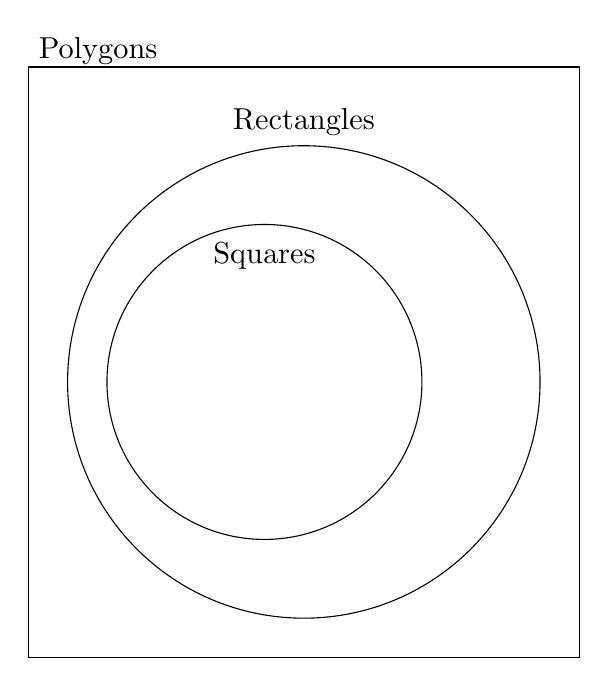
\begin{tikzpicture}[fill=gray]
  \draw (-3.5,-3.5) rectangle (3.5,4.0);
  \draw (-3.5, 4.2) node [above,right] {Polygons};
  \draw (0,0) circle (3) (0,3)  node [above] {Rectangles};
  \draw (-0.5,0) circle (2) (-0.5,1.9)  node [below] {Squares};
\end{tikzpicture}

As the combinations get more complex, we sometimes use shading to
indicate what part we are talking about.  For example, imagine we
wanted all the rectangles with area greater than 5.0 that are not
squares.  The diagram might look like this:

\begin{tikzpicture}[fill=sdkblue]
  \draw (-3.5,-3.5) rectangle (7,4.0);
  \scope
  \clip (0,0) circle (3);
  \fill (3,0) circle (3);
  \fill [white] (-0.5,0) circle (2);
  \endscope
  \draw (-3.5, 4.2) node [above,right] {Polygons};
  \draw (0,0) circle (3) (0,3)  node [above] {Rectangles};
  \draw (-0.5,0) circle (2) (-0.5,1.9)  node [below] {Squares};
  \draw (3,0) circle (3) (3,3)  node [above] {Area > 5.0};
\end{tikzpicture}


\section{Logic}

We use a lot of logic in set theory.  For example, the shaded region
above represents all the polygons for which all the following are
true:
\begin{itemize}
\item It is a rectangle.
\item It is \textit{not} a square.
\item It has an area greater than 5.0.
\end{itemize}

\section{Implies}

In logic, we will often say ``$a$ implies $b$''.  That means ``If the
statement $a$ is true, the statement $b$ is also true.''  For example:
``$p$ is a square'' implies ``$p$ is a rectangle.''\index{implies}

There is notation for this: An arrow in the direction of the implication.

$$p \text{ is a square } \implies p \text{ is a rectangle}$$

Notice that implication has a direction: ``$p$ is a rectangle'' does \textit{not} imply 
``$p$ is a square.''

\section {If and Only If}

If the implication goes both ways, we use ``if and only if''.  This
means the two conditions are equivalent.  For example: ``$n$ is even
if and only if there exists an integer $m$ such that $2m = n$'' \index{if and only if}

There is a notation for this too:

$$p \text{ is even } \iff \text{ there exists an integer } m \text{ such that } 2m = n$$

There is even notation for ``there exists''. It is a backwards capital E:

$$p \text{ is even } \iff \exists m \in \mathbb{Z}  \text{ such that } 2m = n$$

\section {Not}

The not operation flips the truth of an expression:\index{not}
\begin{itemize}
\item If $a$ is true $\text{not}(a)$ is false.

\item If $a$ is false $\text{not}(a)$ is true.
\end{itemize}



\graphicspath{{../../Chapters/linked_list_c/en_US}}
\chapter{Linked Lists}

A linked list is a linear data structure where each element is a
separate object, called a node. Each node holds its own data and the
address of the next node, thus forming a chain-like structure.\index{linked list}

A simple node in a linked list can be represented in C++ as follows:



\begin{lstlisting}[language=C++]
struct Node {
    int data;
    Node* next;
};
\end{lstlisting}

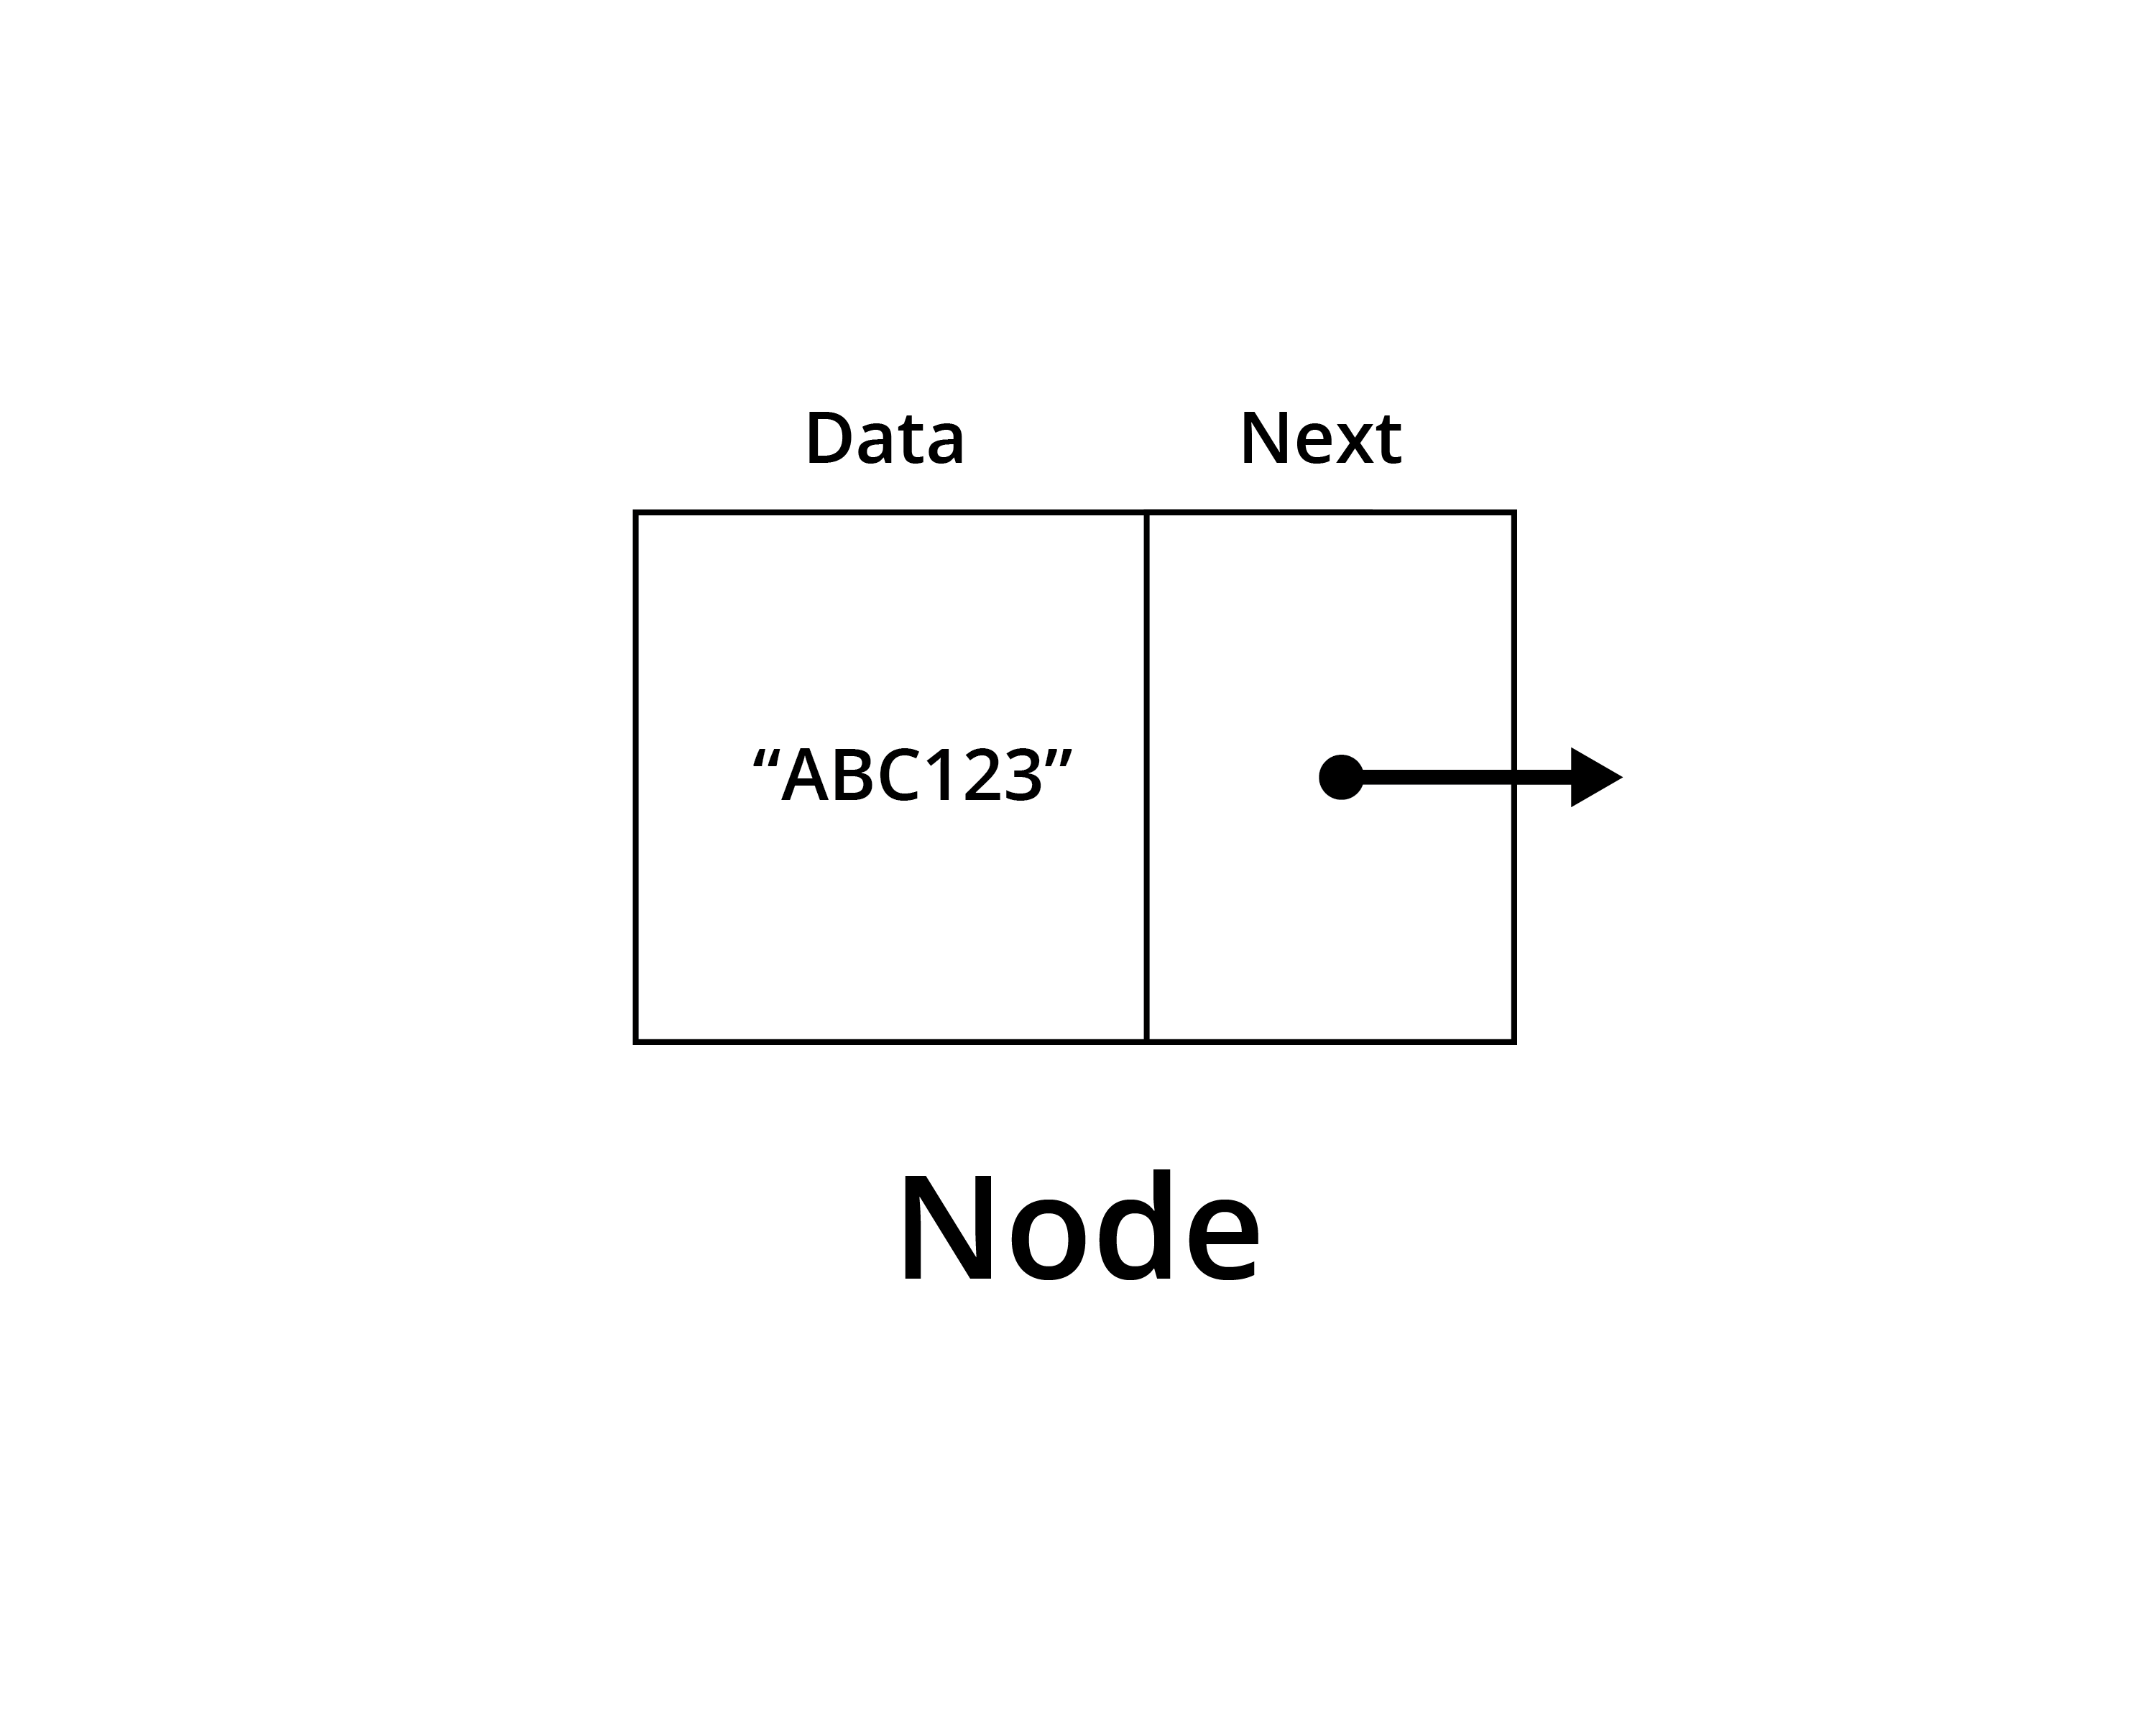
\includegraphics[width=0.5\textwidth]{node.png}


In this structure, 'data' is used to store the data and 'next' is a
pointer that holds the address of the next Node in the list.



Here is a simple example of creating and linking nodes in a linked
list:

\begin{lstlisting}[language=C++]
// Create nodes
Node* head = new Node();
Node* second = new Node();
Node* third = new Node();
\end{lstlisting}

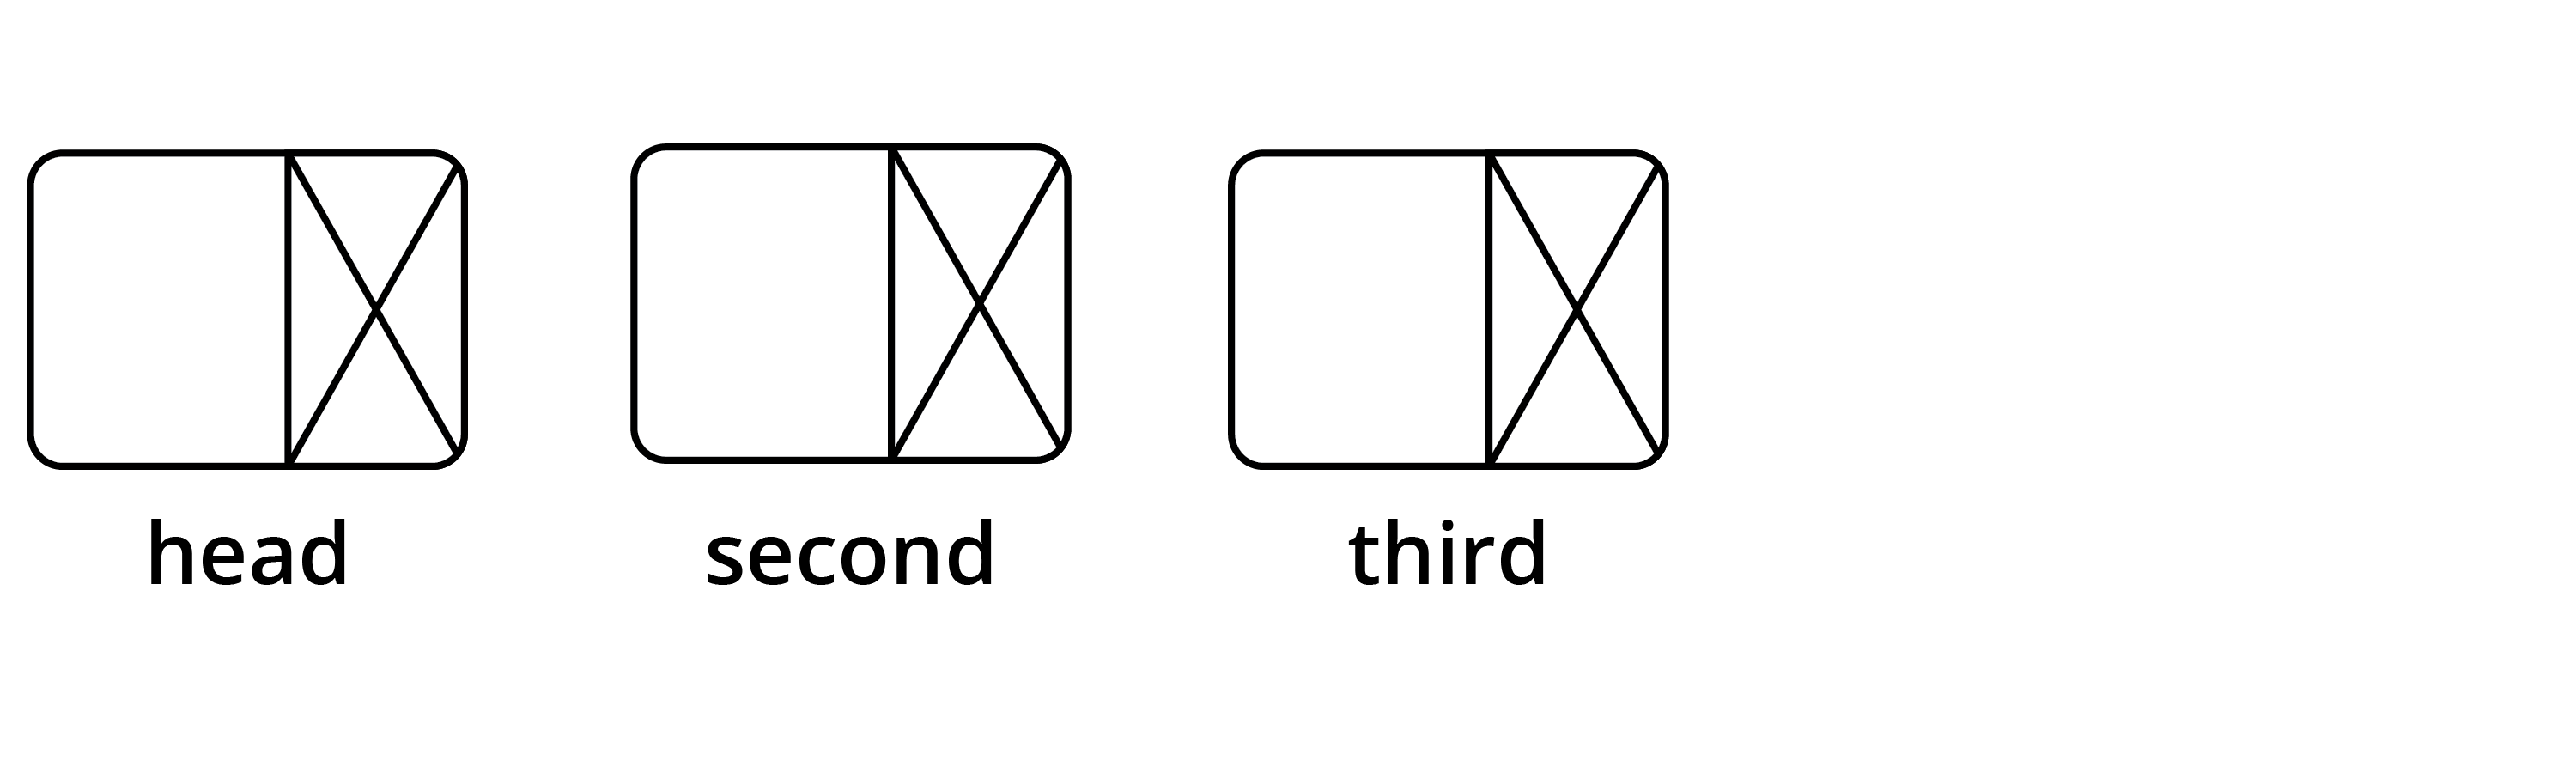
\includegraphics[width=.75\textwidth]{llexample-03.png}

\begin{lstlisting}[language=C++]

// Assign data
head->data = 1;
second->data = 2;
third->data = 3;
\end{lstlisting}

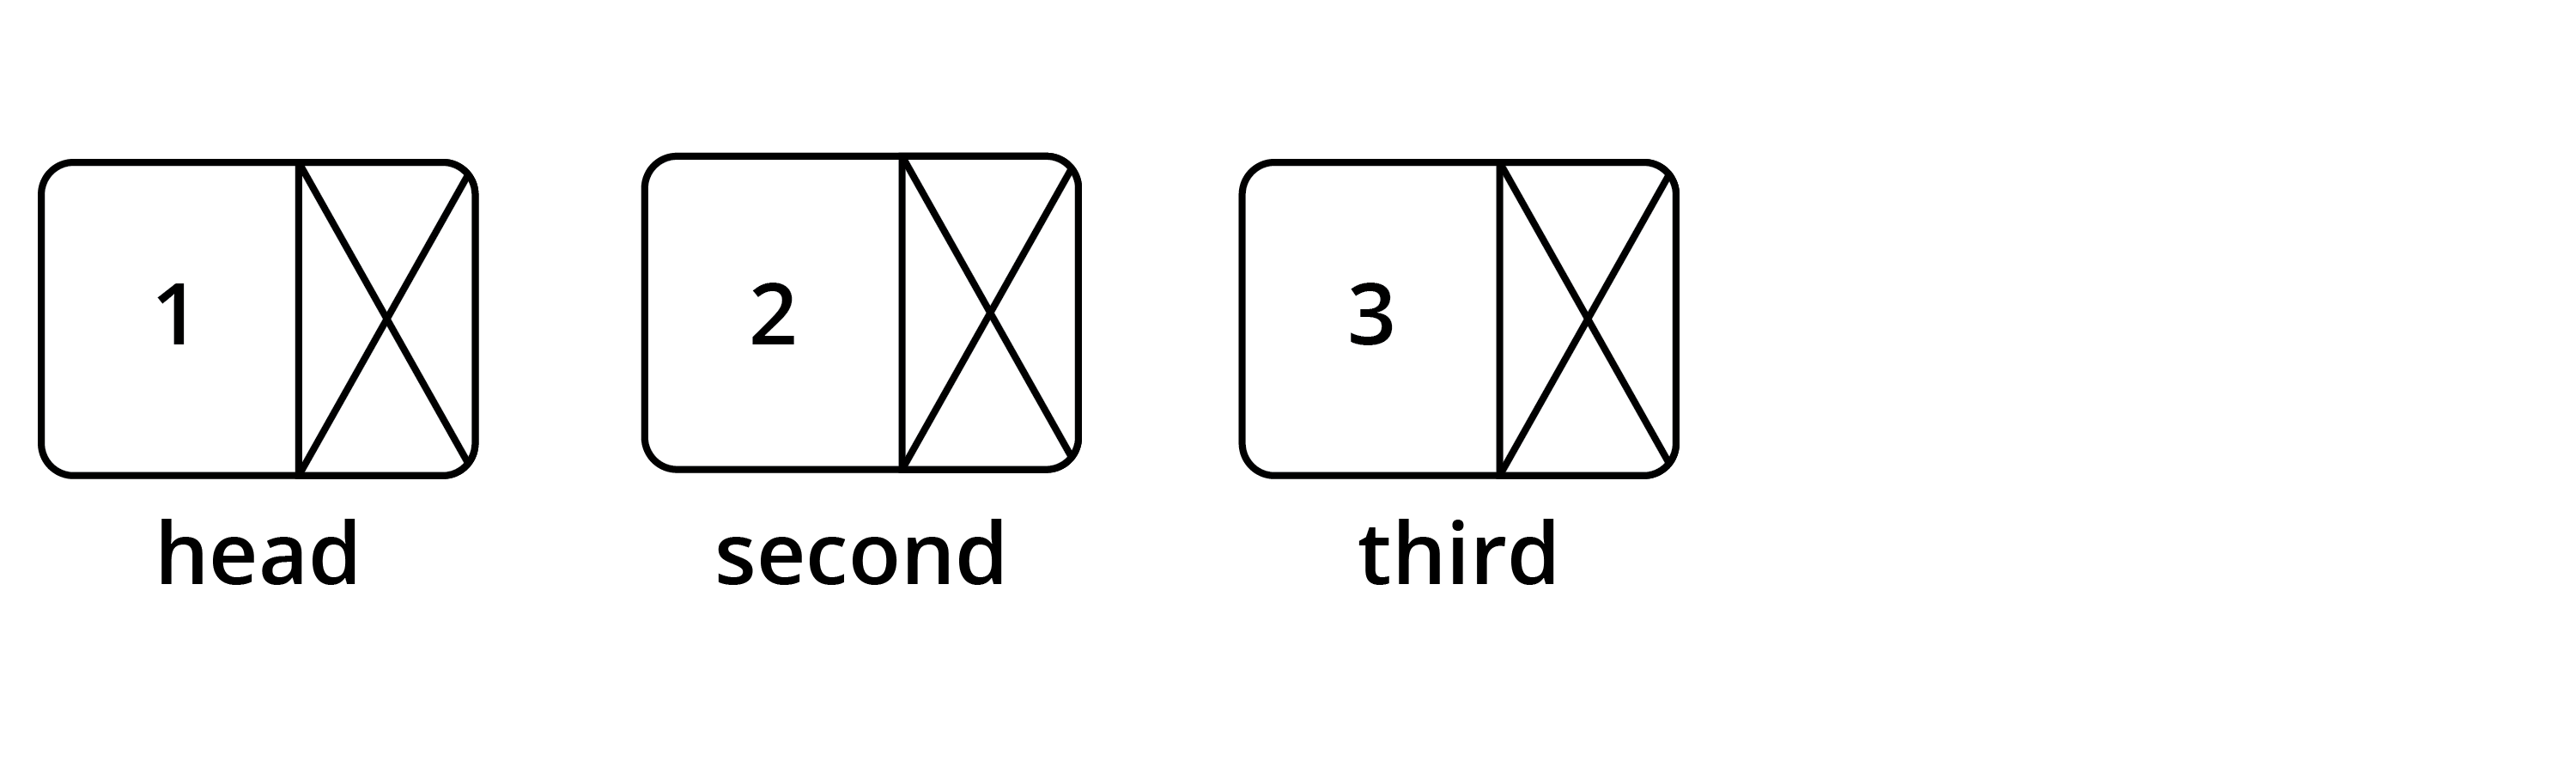
\includegraphics[width=.75\textwidth]{llexample-04.png}

\begin{lstlisting}[language=C++]
// Link nodes
head->next = second;
second->next = third;
third->next = nullptr;  // The last node points to null
\end{lstlisting}


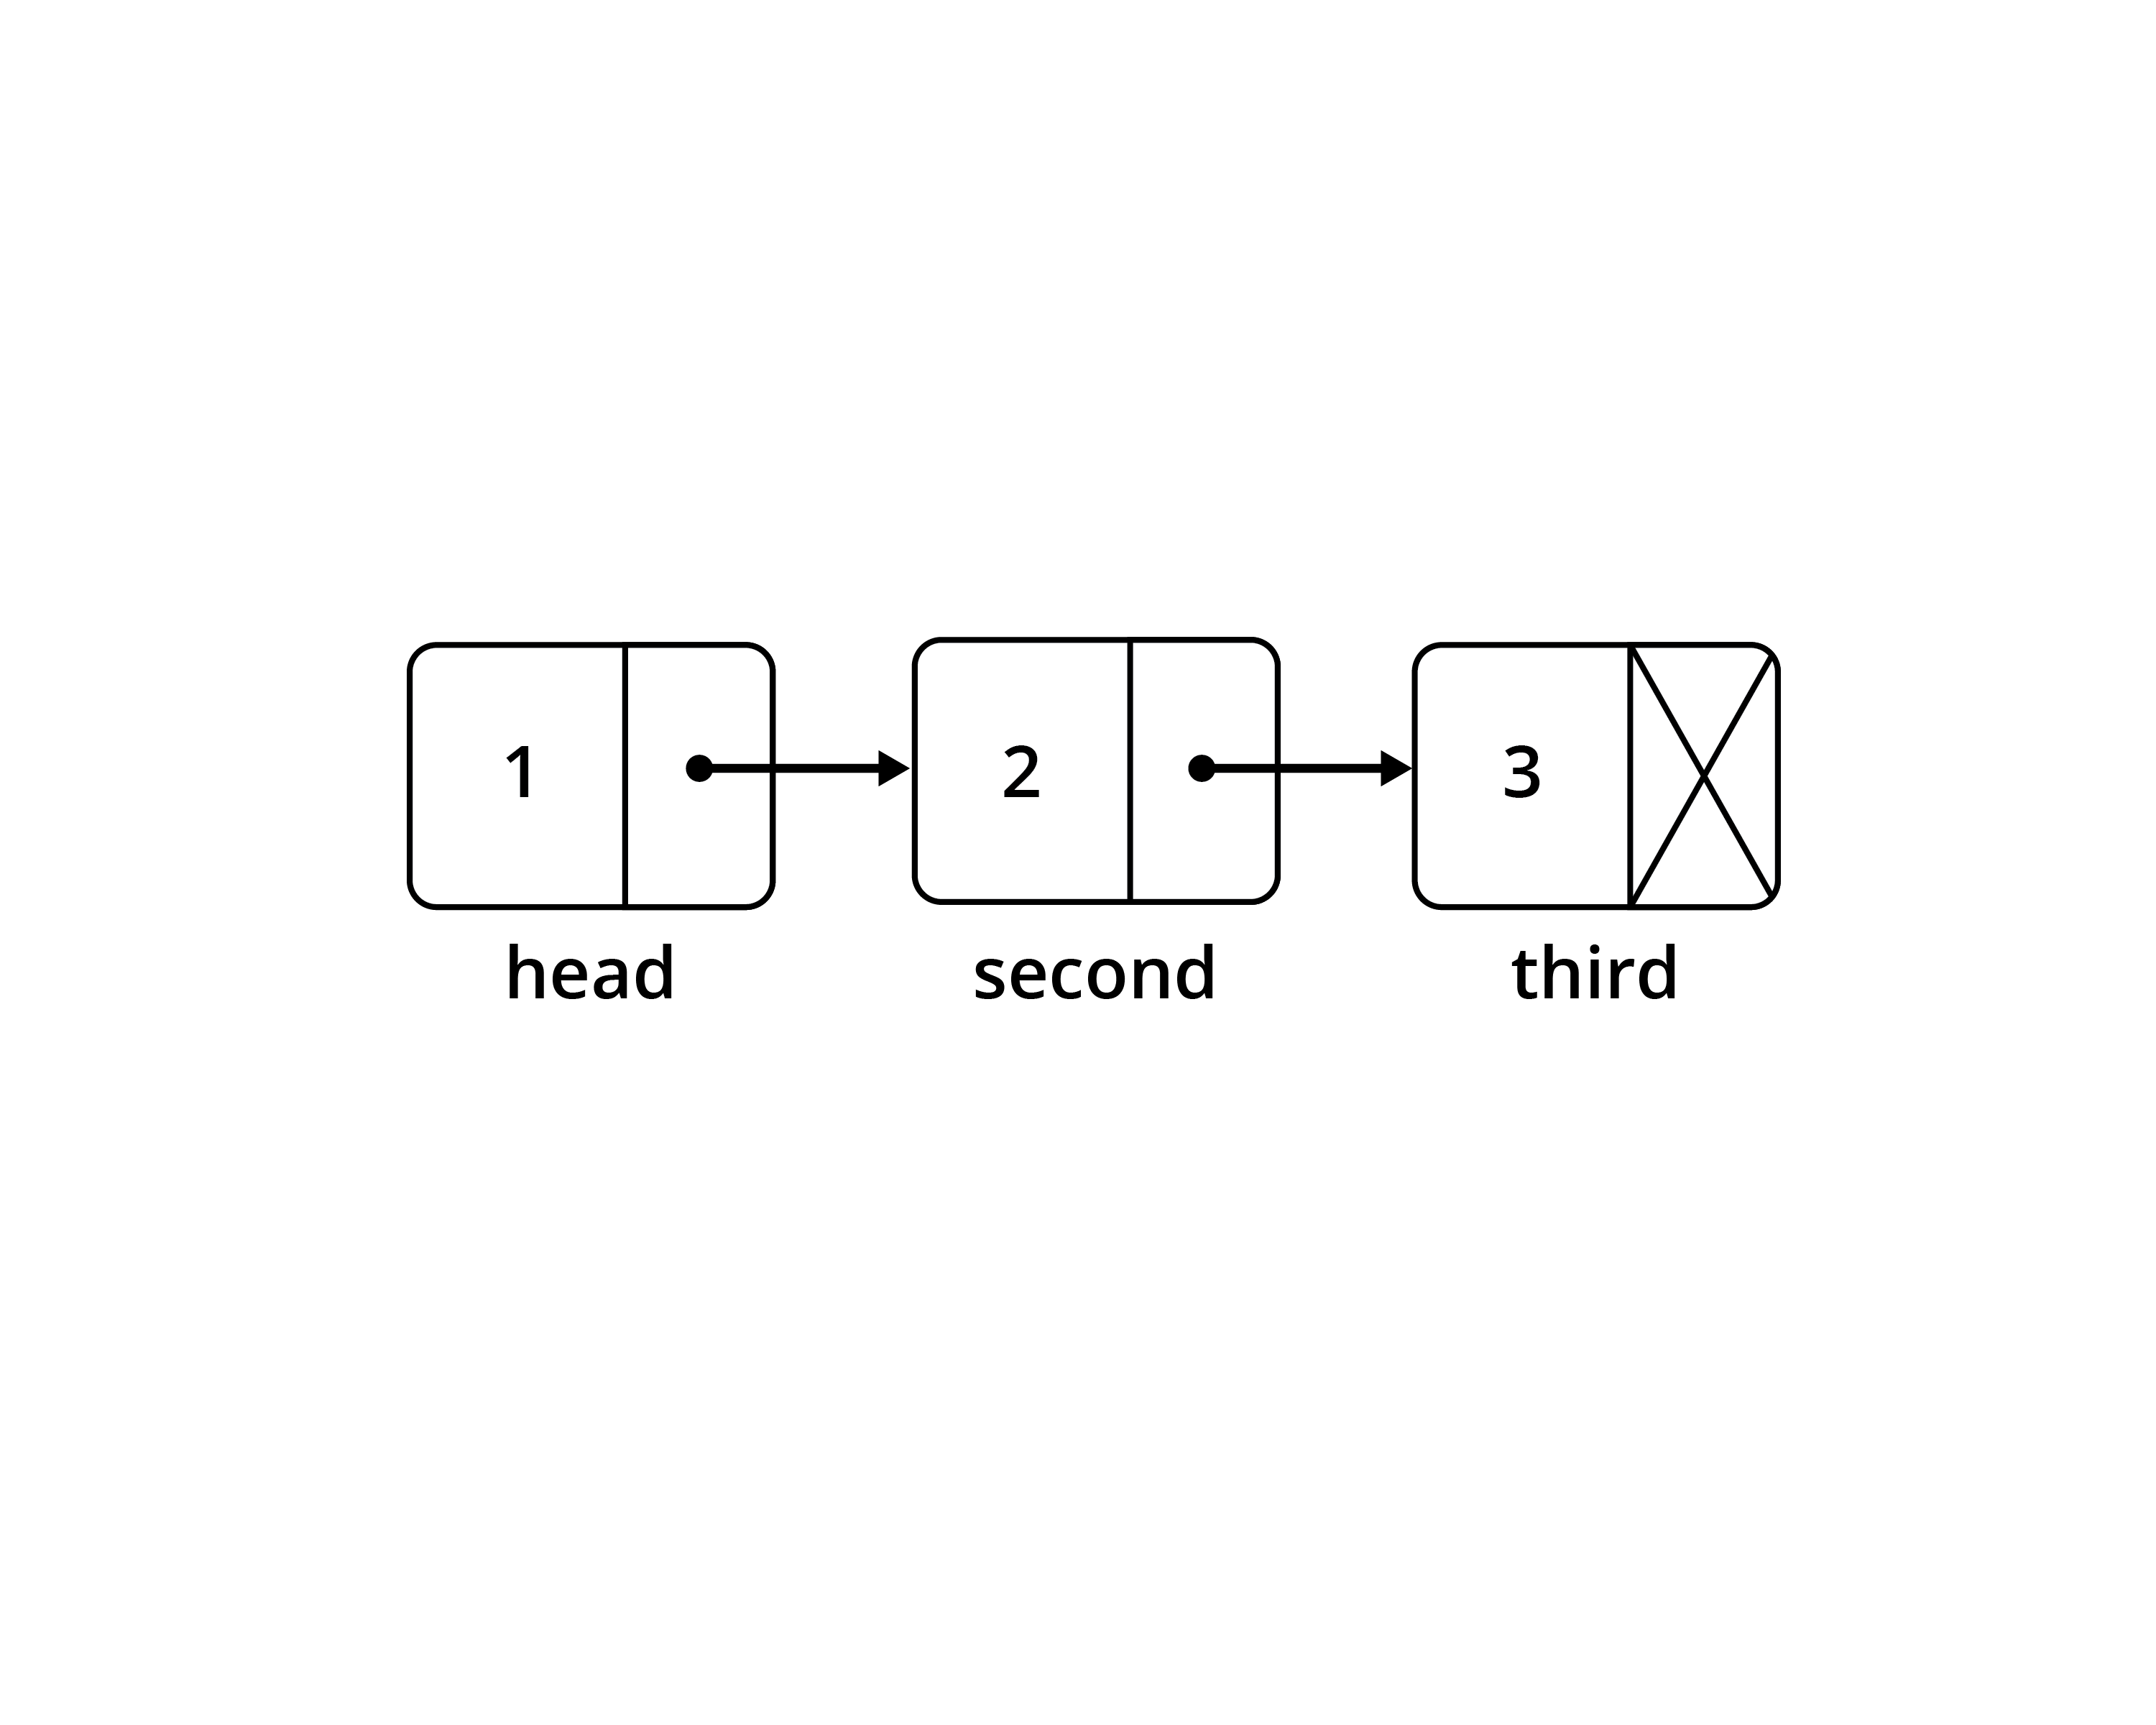
\includegraphics[width=.75\textwidth]{llexample-05.png}



In this example, we first create three nodes using the `new` keyword,
which dynamically allocates memory. We then assign data to the nodes
and link them using the 'next' pointer.

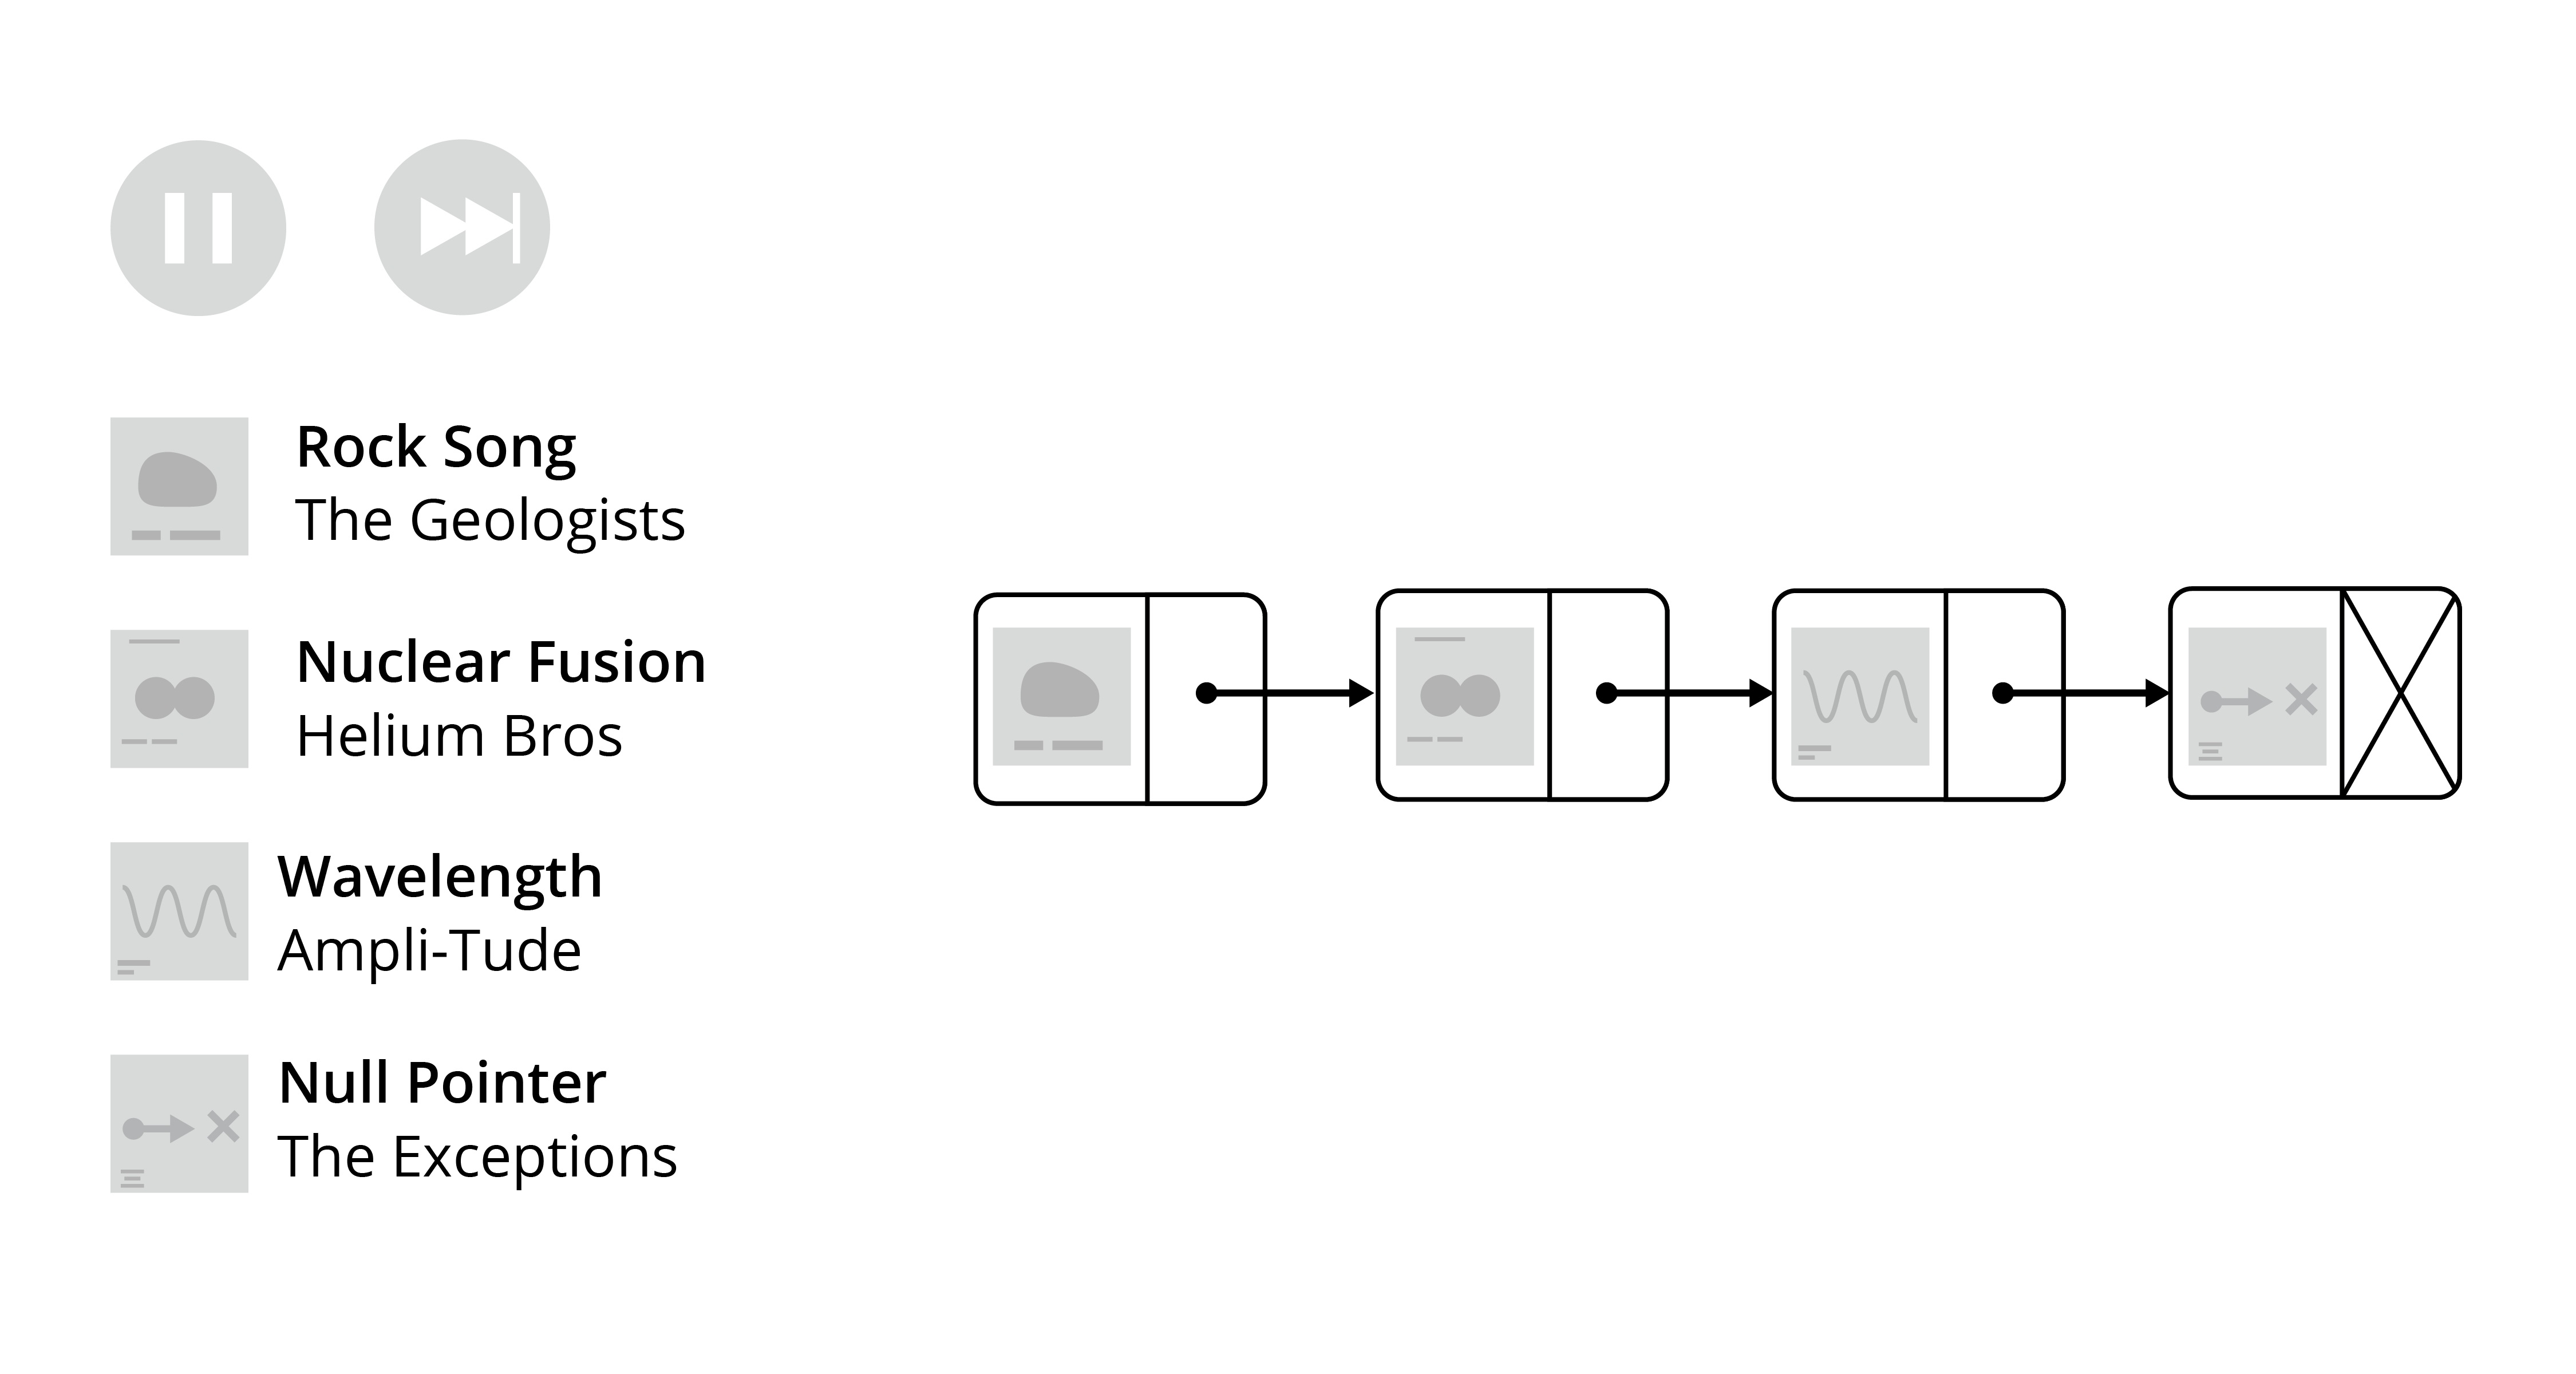
\includegraphics[width=1\textwidth]{playlistCombined.png}

\graphicspath{{../../Chapters/trees/en_US}}
\chapter{Trees}

Trees are one of the most versatile and widely used data structures in computer science. A tree is a hierarchical data structure consisting of nodes, where each node has a value and a set of references to its child nodes. The node at the top of the hierarchy is called the root, and nodes with the same parent are called siblings.

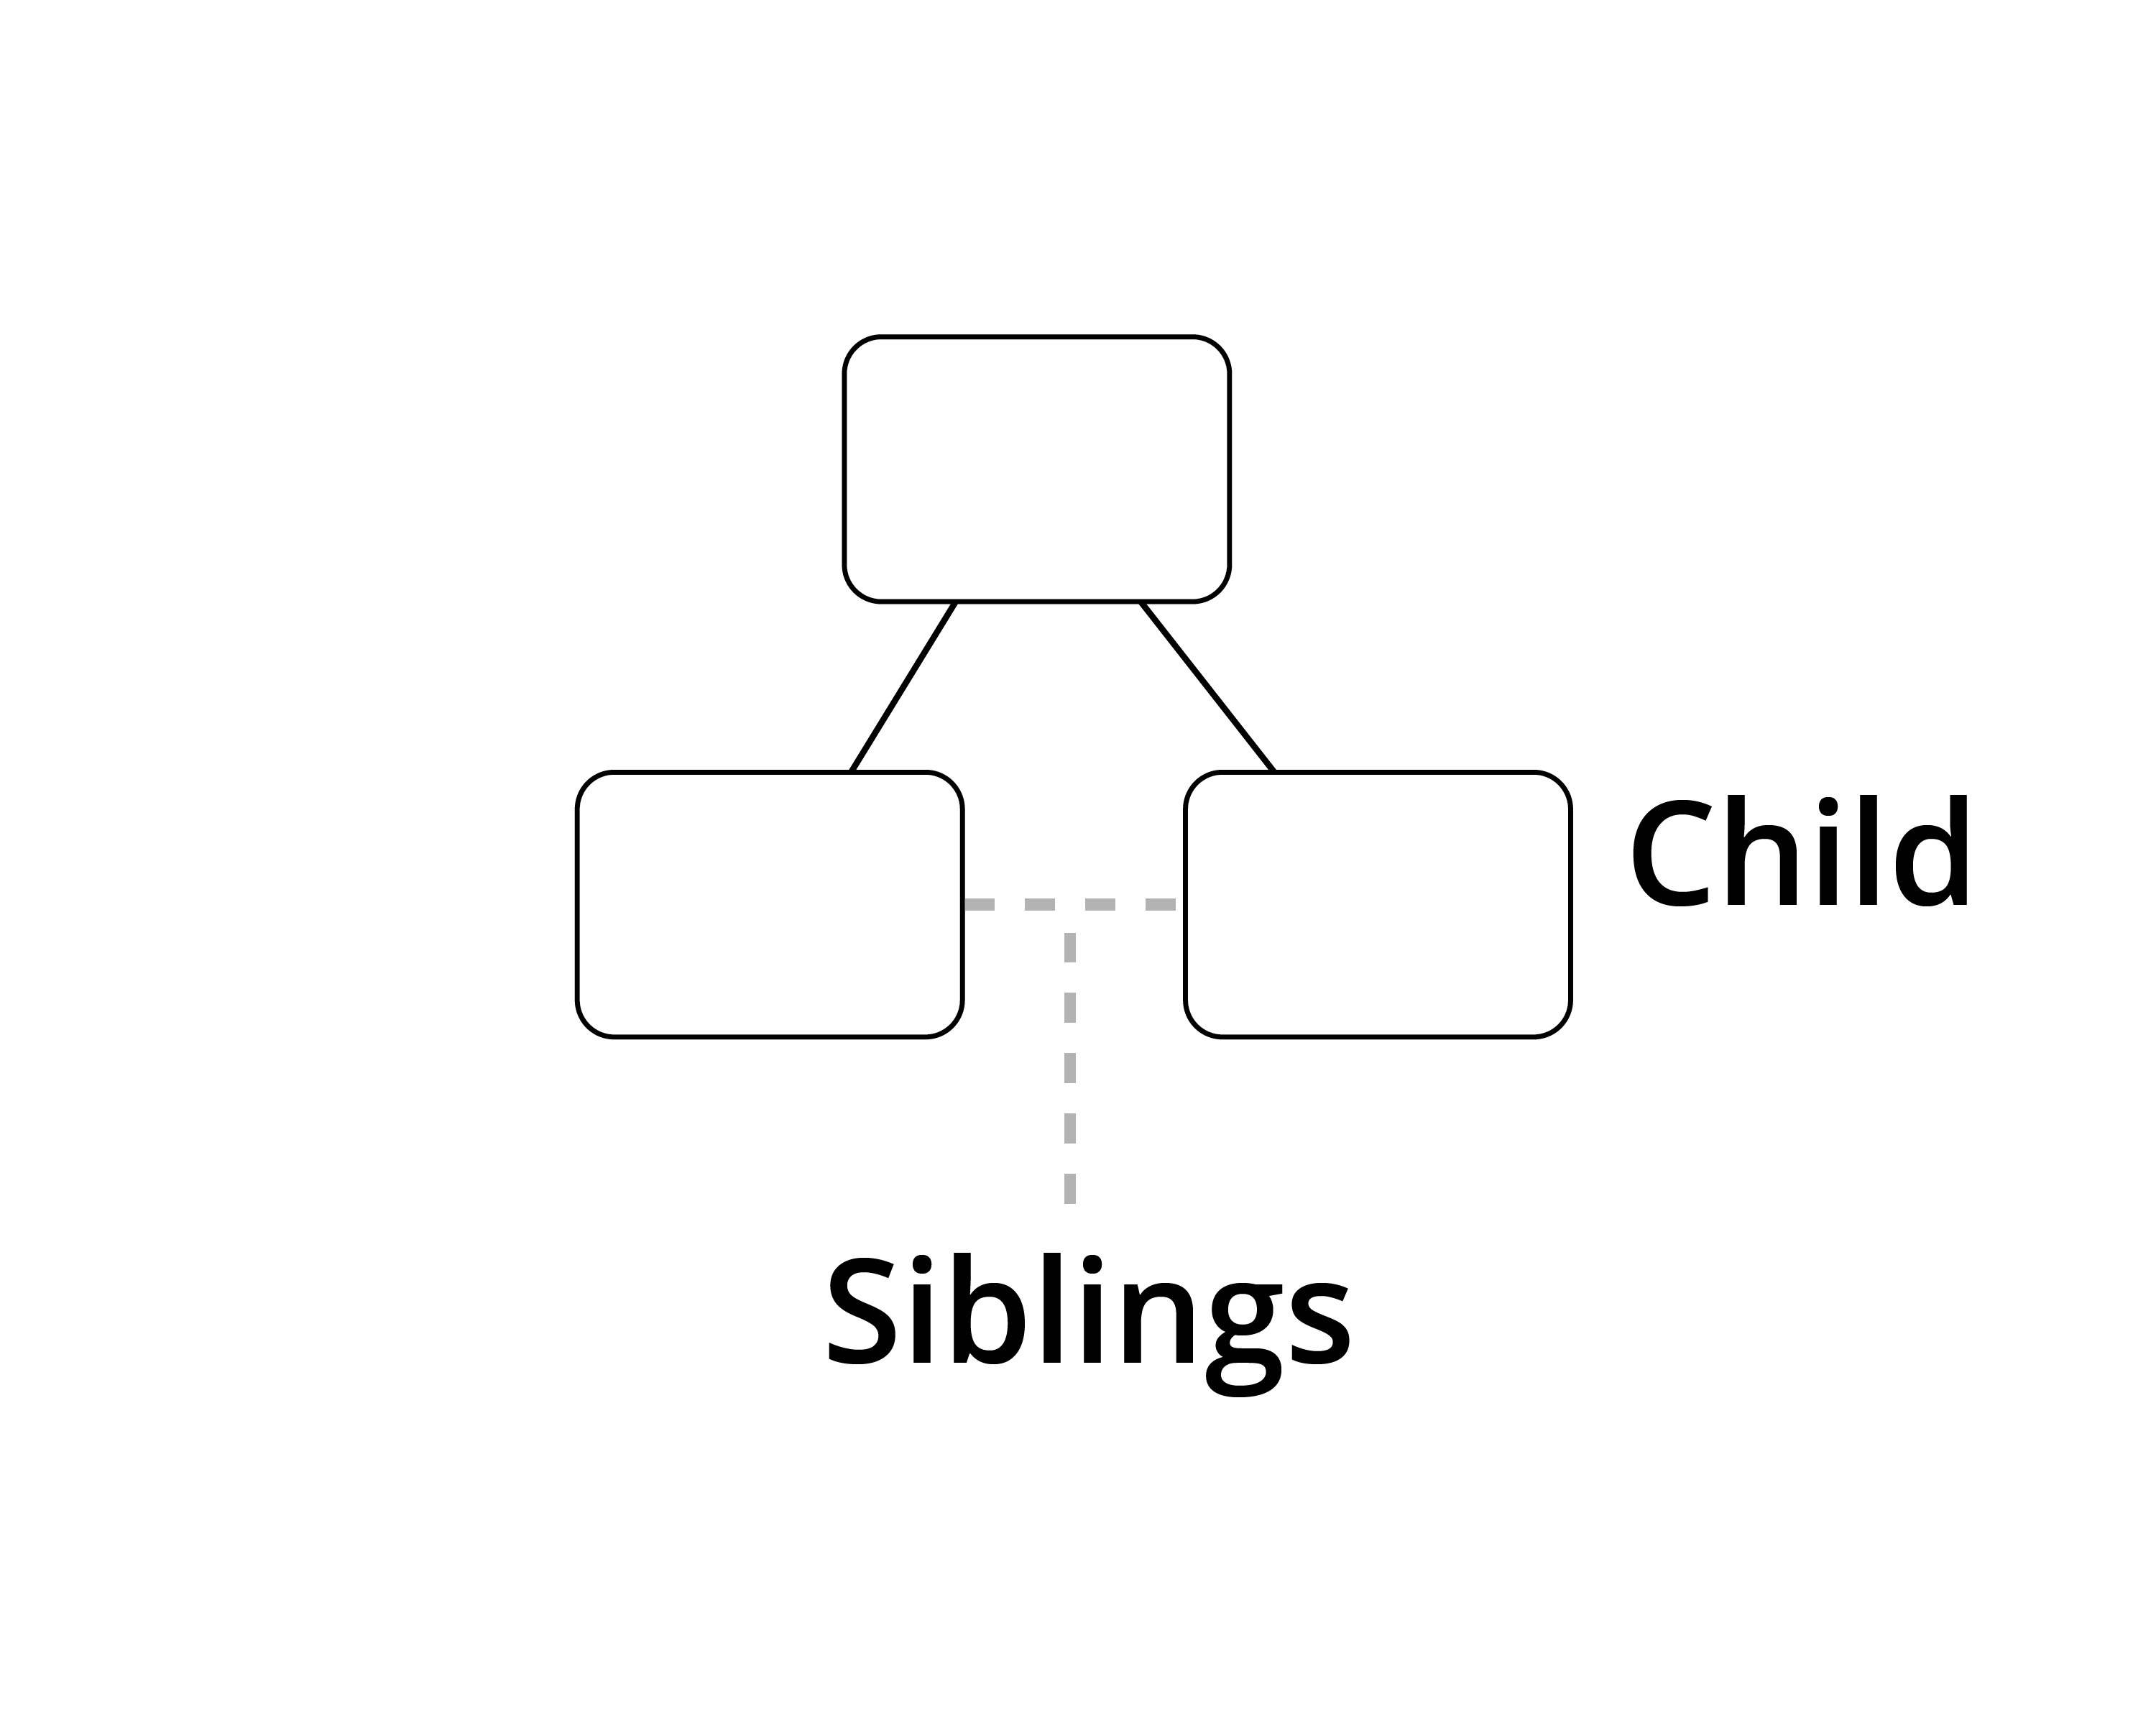
\includegraphics[width=0.75\textwidth]{parentChild.png}

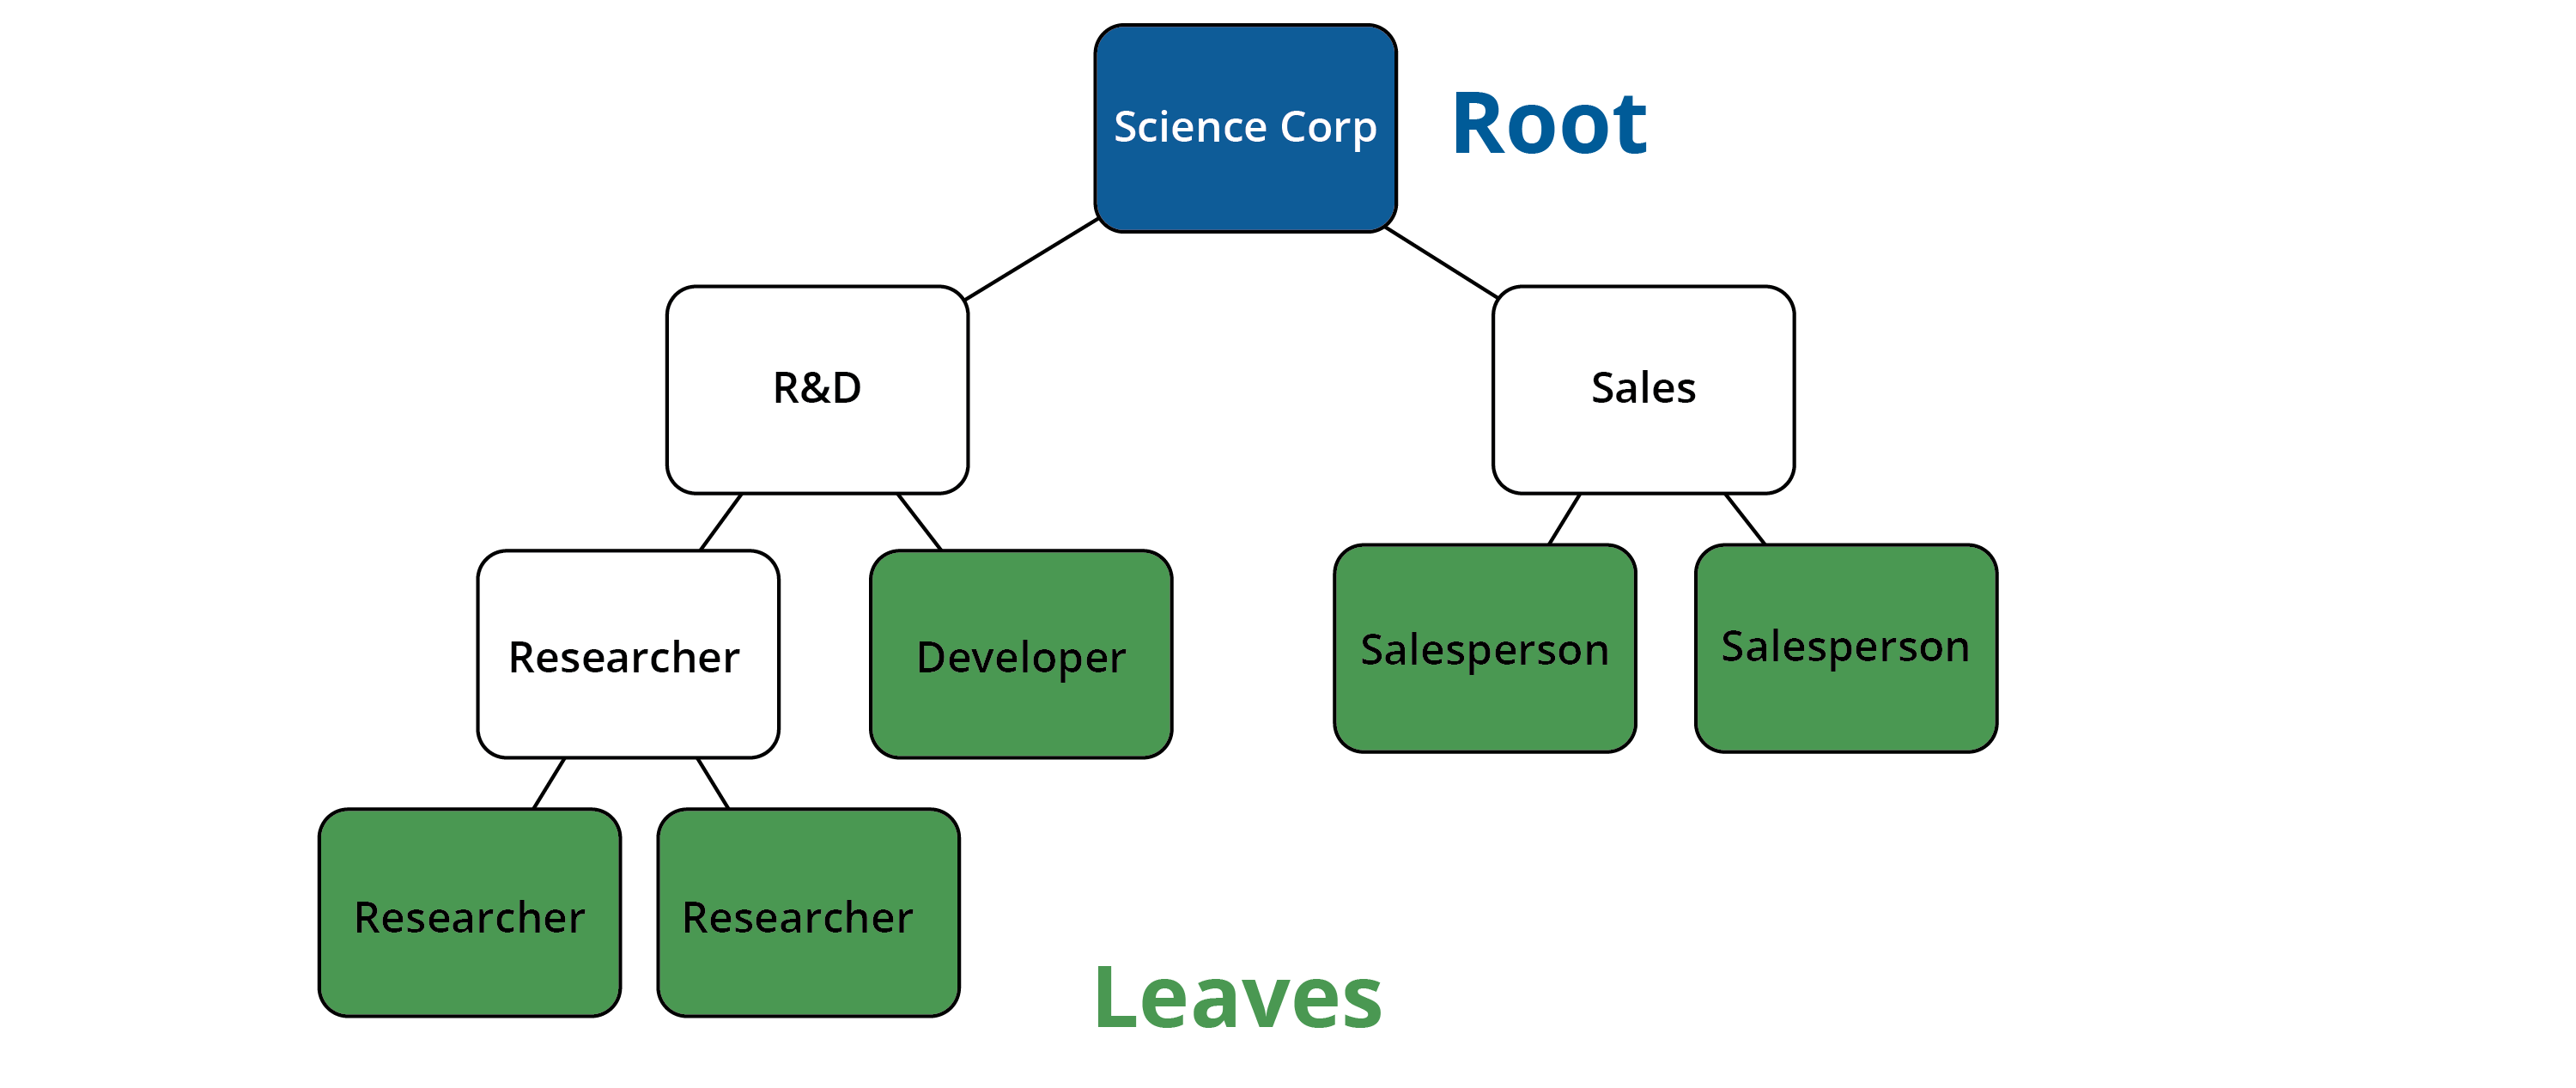
\includegraphics[width=0.75\textwidth]{rootLeaves.png}


The power of trees comes from their ability to represent complex relationships between objects, while providing efficient operations for accessing and modifying those objects. Trees can be used to represent hierarchical relationships, to organize data for quick search and insertion, and to manage sorted lists of data, among other uses.

In this chapter, we will delve into the details of the tree data structure. We will start with the definition and properties of trees, including the key concepts of roots, nodes, children, siblings, leaves, and levels. We will then introduce binary trees, a specific type of tree where each node has at most two children, which are referred to as the left child and the right child.

We will explore the various ways to traverse a tree, including depth-first and breadth-first traversals, and discuss the applications and efficiencies of these methods. We will then cover binary search trees, a variant of binary trees that allows for fast lookup, addition, and removal of items.

Then, we'll take a look at balanced search trees, such as AVL trees and red-black trees, which automatically keep their height small to guarantee logarithmic time complexity in the worst case for search, insert, and delete operations.

Finally, we will explore more advanced topics such as B-trees, tries, and suffix trees, which have applications in databases, file systems, and string algorithms.

By the end of this chapter, you will have a deep understanding of the tree data structure, its variants, and their uses. Armed with this knowledge, you'll be able to choose the right tree structure for your data and implement it effectively in your software.

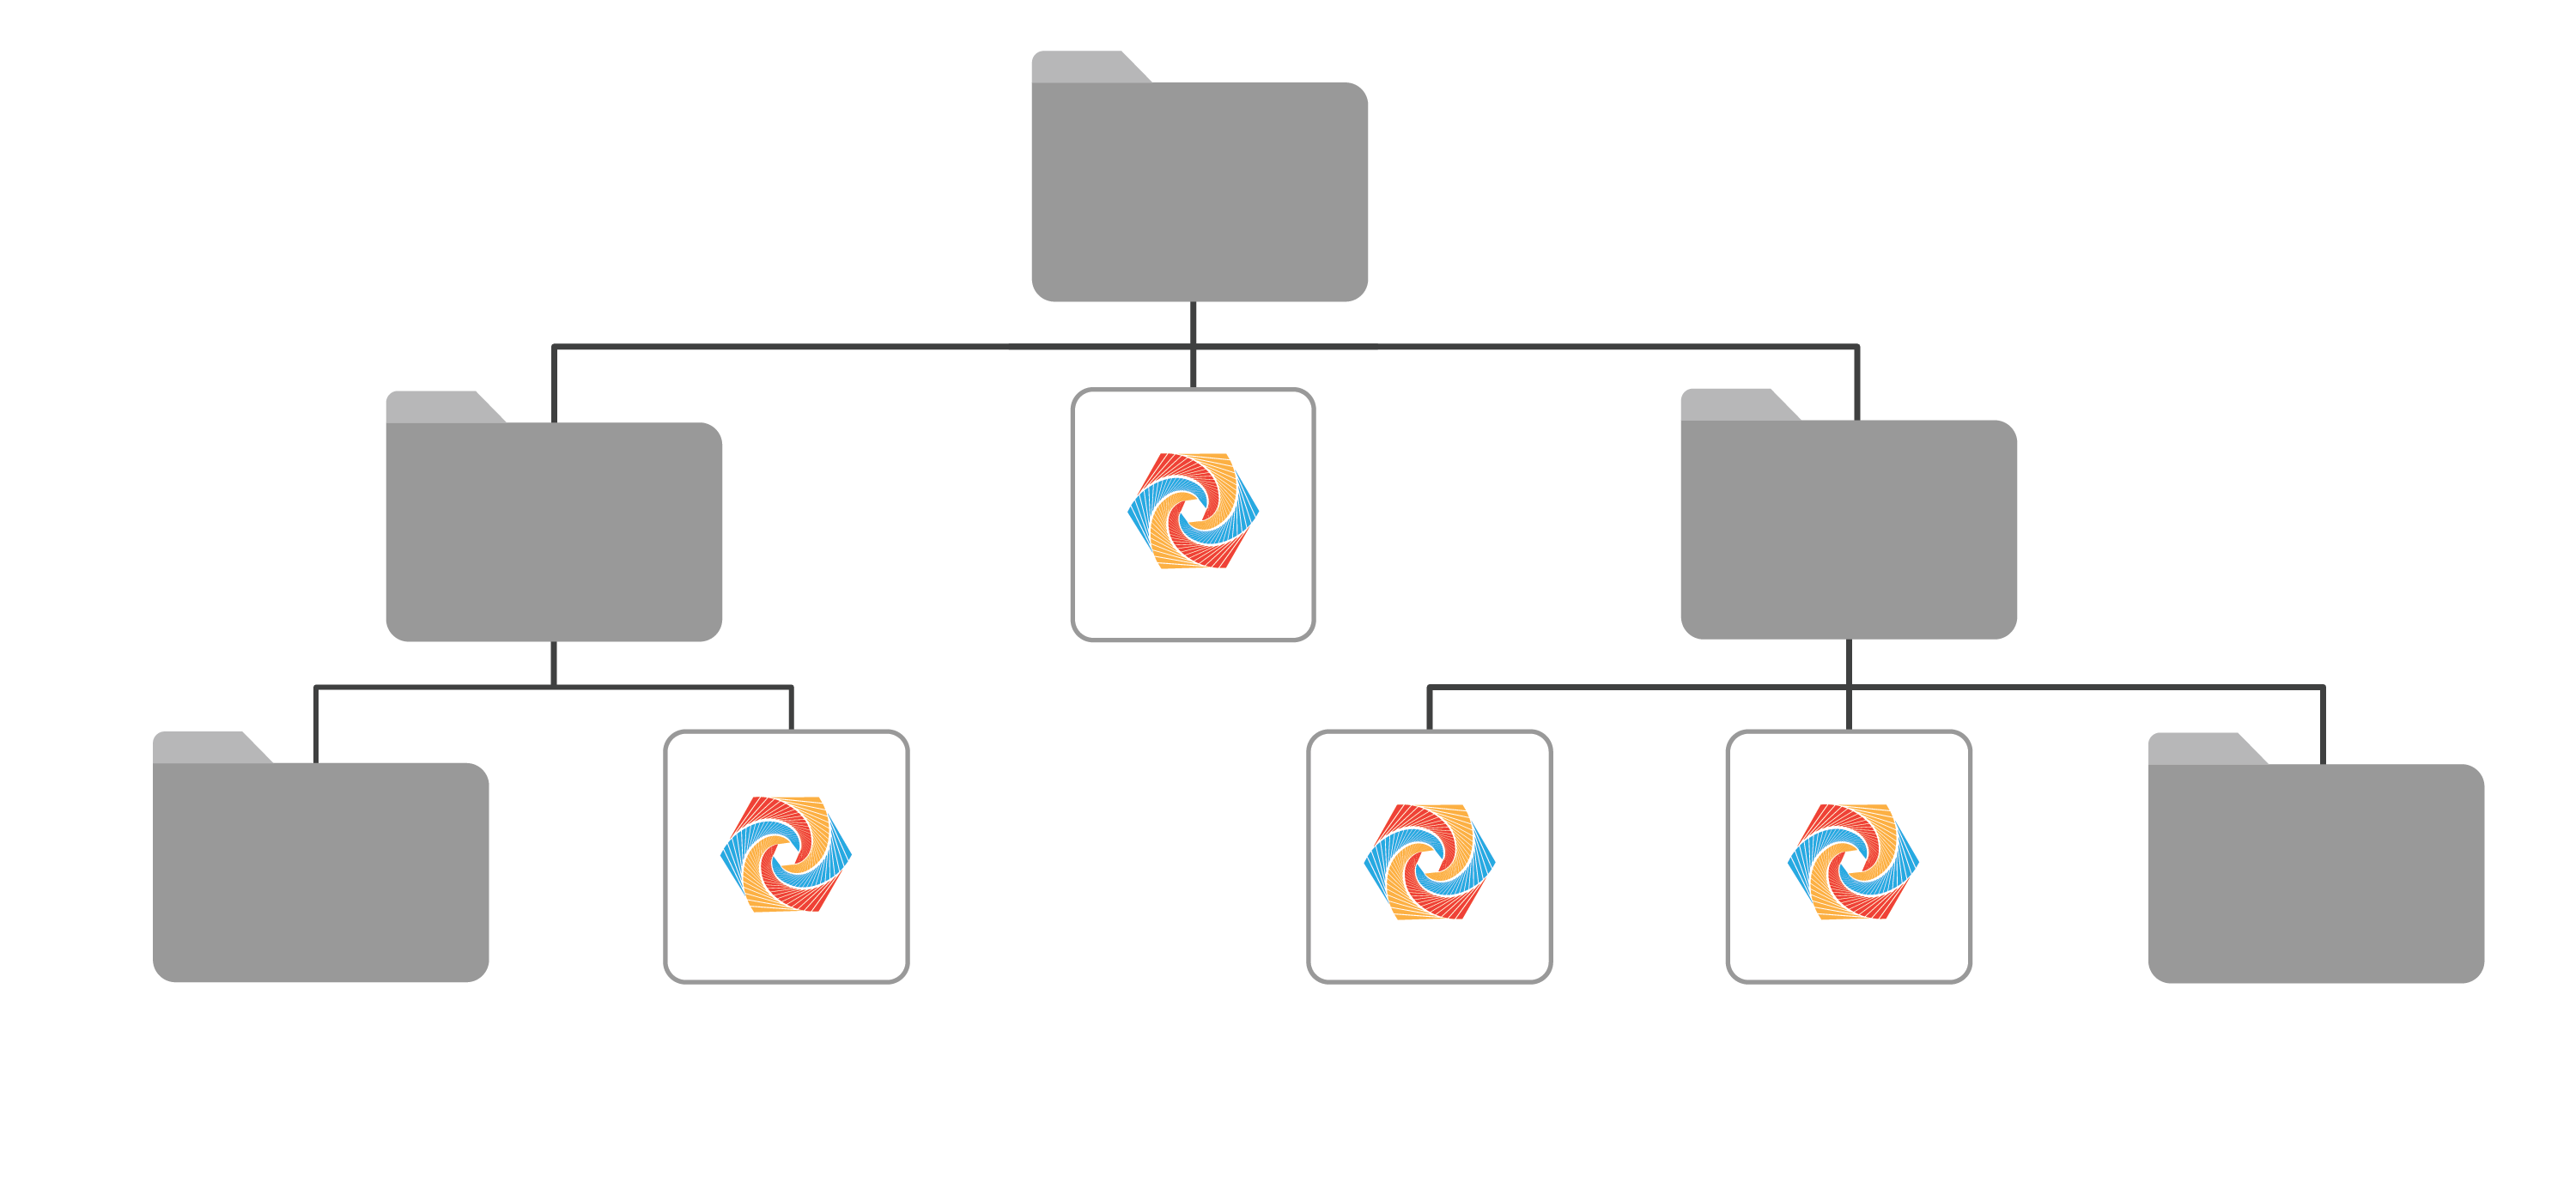
\includegraphics[width=1\textwidth]{fileStructure.png}



\graphicspath{{../../Chapters/searching_trees/en_US}}
\chapter{Searching Trees}

\graphicspath{{../../Chapters/hash_tables/en_US}}
\chapter{Hash Tables}

A hash table, also known as a hash map, is a data structure that
implements an associative array abstract data type, a structure that
can map keys to values. It uses a hash function to compute an index
into an array of buckets or slots, from which the desired value can be
found.\index{hash table}

\section{Structure of a Hash Table}

A hash table is composed of an array (the 'table') and a hash
function. The array has a predetermined size, and each location (or
'bucket') in the array can hold an item (or several items if
collisions occur, as will be discussed later). The hash function is a
function that takes a key as input and returns an integer, which is
then used as an index into the array.\index{hash function}

\section{Inserting and Retrieving Data}

When inserting a key-value pair into the hash table, the hash function
is applied to the key to compute the index for the array. The
corresponding value is then stored at that index.

When retrieving the value associated with a key, the hash function is
applied to the key to compute the array index, and the value is
retrieved from that index.

\section{Handling Collisions}

A collision occurs when two different keys hash to the same
index. There are several methods for handling
collisions:\index{collisions in hash tables}

\begin{itemize}
    \item \textbf{Chaining (or Separate Chaining)}: In this method,
      each array element contains a linked list of all the key-value
      pairs that hash to the same index. When a collision occurs, a
      new key-value pair is added to the end of the list.
    \item \textbf{Open Addressing (or Linear Probing)}: In this
      method, if a collision occurs, we move to the next available
      slot in the array and store the key-value pair there. When
      looking up a key, we keep checking slots until we find the key
      or reach an empty slot.
\end{itemize}

\section{Time Complexity}

In an ideal scenario where hash collisions do not occur, hash tables
achieve constant time complexity $O(1)$ for search, insert, and delete
operations. However, due to hash collisions, the worst-case time
complexity can become linear $O(n)$, where $n$ is the number of keys
inserted into the table.

Using good hash functions and collision resolution strategies can
minimize this issue and allow us to take advantage of the hash table's
efficient average-case performance.


\graphicspath{{../../Chapters/sorting/en_US}}
\chapter{Sorting Algorithms}

Sorting is a fundamental problem in computer science that has been extensively studied for many years. Sorting is the process of arranging items in ascending or descending order, based on a certain property. In the realm of algorithms, sorting generally refers to the process of rearranging an array of elements according to a specific order. This order could be numerical (ascending or descending) or lexicographical, depending on the nature of the elements.

Sorting algorithms form the backbone of many computer science and software engineering tasks. They are used in a myriad of applications including, but not limited to, data analysis, machine learning, graphics, computational geometry, and optimization algorithms. Thus, understanding these algorithms, their performance characteristics, and their suitability for specific tasks is crucial for anyone venturing into these fields.

This chapter will introduce several sorting algorithms, ranging from elementary methods like bubble sort and insertion sort to more advanced algorithms such as quicksort, mergesort, and heapsort. We will study these algorithms in terms of their time and space complexity, stability, and adaptability, among other characteristics. By the end of this chapter, you should have a solid understanding of how different sorting algorithms work and how to choose the appropriate algorithm for a specific context.

The knowledge of sorting algorithms not only helps in writing efficient code but also strengthens your problem-solving ability and analytical thinking, which are essential skills for succeeding in any technical interview. Let's dive into this fascinating world of sorting algorithms.

%%%%%%%%%%%%%%%%%%%%%%%%%%%%%%%%%
%% Bookfooter.tex by Aaron Hillegass
%% Nov 8, 2020

\appendix

\chapter{Answers to Exercises}
\shipoutAnswer

\bibliography{references}

\printindex

\end{document}